\chapter{考察}
\section{緩和項の相対評価}
\begin{figure}[h]
  \centering
  \includegraphics[width=10cm]{./chap4/fig/comparison.png}
  \caption{ビーム照射中の緩和効果の比較}
\end{figure}
(グラフは和の形で表記していることがわかるように修正する)
レーザ照射下の偏極緩和項は加速器によるビーム照射の有無にかかわらず存在する。
\\
$\downarrow \bf{この部分はわかりにくいので後ほど書き直す}$\\
・強度効果を定数にした話(多くの仮定をしているので単純に今回はこう考えました、という話)\\
強度効果による緩和項は微分方程式中で定数で置いていたため、グラフ中でもビーム照射中のみ一定に寄与している。
本論文では強度効果は結晶温度に比例すると仮定している。
結晶温度はナフタレンの比熱とビームから与えられた熱量の積となる。
ナフタレンの比熱と温度は図$\ref{C_T}$のような関係を持つことがわかっており$\cite{Chem}$、$0 [K]<T<273 [K]$の範囲で比例関係にあるとみなすことができる。
したがって、ビーム照射により一定の熱量を与え続けた場合、標的温度の上昇に伴いナフタレンの温度上昇に必要な熱量も増加し、ある時点で温度は平衡に達すると考えた。
温度が平衡に達すると強度効果も固定値となるため、温度が平衡に達するまでの上昇を$\rm{exp}(\frac{t}{\gamma})$として補正したうえで強度効果を定数として微分方程式に取り込んだ。
ただし、本論文ではビーム強度によって達する平衡温度と平衡に達するまでの時間が異なることを考慮できていないため、今後改善が必要である。
\begin{figure}[h]
  \centering
  \includegraphics[width=10cm]{./chap4/fig/C_T.png}
  \caption{ナフタレンの飽和圧力におけるモル熱容量$\cite{Chem}$}
  \label{C_T}
\end{figure}


\section{長時間・大強度ビーム照射時の減偏極予想}
\begin{figure}[h]
  \centering
  \includegraphics[width=10cm]{./chap4/fig/longtime.png}
  \caption{長時間・大強度ビーム照射時の減偏極予想}
\end{figure}
本論文における最適パラメータを用いて、各ビーム強度で長時間ビーム照射を行った時の減偏極の様子を計算した。
このグラフと先ほどの緩和項比較のグラフから、長時間ビーム照射時の減偏極は積分項の効果が支配的となることがわかる。
また、ビーム強度$1 \times 10^7$ [cps]以上では24時間で偏極度が5割を下回ると推定できる。
今後のビーム照射試験時はビーム強度および照射時間を設定する際にこれらの推定が判断材料となると考えられる。


% \chapter{${}^3$Heの偏極生成と偏極度の絶対値較正}
% 第3章で述べた偏極$^3$He標的装置を用いて、$^3$Heの偏極生成および$^3$He偏極度測定を行った。またRbのESR周波数シフト測定を行い、$^3$He偏極度の絶対値を求めるとともに、AFP-NMR法により得られるNMR信号の較正を行った。本章では、それらの測定結果について述べる。

% %%%% 4.1 %%%%
%  \section{${}^3$He偏極生成}
% 本研究での$^3$He偏極生成には、標的セル製作装置で製作したKukiセルを用いた。$^3$Heの偏極生成では、オーブン温度を$160$℃に設定し、レーザー出力$20~{\rm W}$で光ポンピングを行った。3.2.3節で述べたように、本研究で用いた半導体レーザーは最大出力が$30~{\rm W}$であるが、ファイバー端の部分での発熱が確認されたため、安全面を考慮し出力を少し落として光ポンピングを行った。\\
%  $^3$Heの偏極生成の時間変化は、1時間毎にNMR測定を行うことで確認した。NMR測定時の測定系の条件を表\ref{NMR_cond}に示す。
% %
% \begin{table}[htbp]
%  \caption{NMRの測定条件}
%  \centering
%   \begin{tabular}{|c|c|} \hline
% 項目 & 設定値 \\ \hline \hline
% 静磁場掃引範囲 & $1.24~{\rm mT}$〜$2.96~{\rm mT}$ \\
% 掃引速度$dB/dt$ & $0.095~{\rm mT/s}$ \\
% RF周波数$f$ & $87.0~{\rm kHz}$ \\
% 共鳴磁場$B_0$ & $2.68~{\rm mT}$ \\
% RFの大きさ$B_1$ & $2.5 \times 10^{-3}~{\rm mT}$ \\ \hline 
%   \end{tabular}
%  \label{NMR_cond}
% \end{table}
% %

% %% 4.1.1 %%
%   \subsection{偏極発展}
% 光ポンピングによる$^3$He偏極度の時間変化(偏極発展)は、式(\ref{P_3He_final})で示したように
% %
% \begin{equation}
%  {P}_{\rm ^3He} = \overline{P}_{\rm Rb} \frac{\gamma_{\rm SE}}{\gamma_{\rm SE}+\Gamma_{\rm ^3He}} \left[ 1-e^{-(\gamma_{\rm SE}+\Gamma_{\rm ^3He})t} \right]
%  \label{P_3He_final2}
% \end{equation}
% %
% と書ける。また十分時間が経過した時($t \to \infty$)の$^3$He原子核の偏極度$\overline{P}_{\rm ^3He}$は、$X$-factorを考慮すると式(\ref{P_3He_X})で示したように
% %
% \begin{eqnarray}
%  \overline{P}_{\rm ^3He} &=& \overline{P}_{\rm Rb} \frac{\gamma_{\rm SE}}{\gamma_{\rm SE}(1+X)+\Gamma_{\rm ^3He}} \nonumber \\
%  &=& \overline{P}_{\rm Rb} \frac{\gamma_{\rm SE}}{\gamma_{\rm SE}+\Gamma_{\rm ^3He}'} 
%  \label{P_3He_X2}
% \end{eqnarray}
% %
% となる。ここで、$\Gamma_{\rm ^3He}' = X \cdot \gamma_{\rm SE}+\Gamma_{\rm ^3He}$はRb蒸気と$^3$He原子核との相互作用も考慮した$^3$He原子核の偏極緩和率である。また偏極発展における立ち上がりの時定数$\tau_{\rm build}$は、
% %
% \begin{equation}
%  \tau_{\rm build} = \frac{1}{\gamma_{\rm SE}+\Gamma_{\rm ^3He}'}
%  \label{tau_build}
% \end{equation}
% %
% と表される。よって$^3$Heの偏極発展を測定し、$\tau_{\rm build}$の値が求まれば、Rb原子と$^3$He原子核のスピン交換率$\gamma_{\rm SE}$および$^3$He原子核の偏極緩和率$\Gamma_{\rm ^3He}'$の和を求めることができる。\\
%  Kukiセルを用いた場合の典型的な$^3$Heの偏極発展の測定結果を図\ref{NMR_build}に示す。図\ref{NMR_build}における実線は、図中に示された式(式(\ref{P_3He_final2})と同様の形)でフィッティングした結果である。また3.1節で述べたように、今回使用したKukiセルはポンピング部と、NMR信号を検出するためのピックアップコイルが設置されている標的部をもつダブルセル構造である。よって、偏極発展を開始してから偏極した$^3$He原子核が標的部に達するまでに時間差が生じる。故に、厳密には偏極発展開始直後における$^3$He偏極度の時間変化は式(\ref{P_3He_final2})と一致しない。以上の理由から、図\ref{NMR_build}の$t \sim 0.5~{\rm h}$における点はフィッティングの範囲に含めないようにした。フィッティングの結果、到達信号強度$V_{\rm max}$および発展の時定数$\tau_{\rm build}$は
% %
% \begin{eqnarray}
%  V_{\rm max} &=& 204.3 \pm 3.4~[{\rm mV}] \\
%  \tau_{\rm build} &=& 7.43 \pm 0.36~[{\rm h}]
% \end{eqnarray}
% %
% となった。

% \begin{figure}[tbp]
%  \centering
%  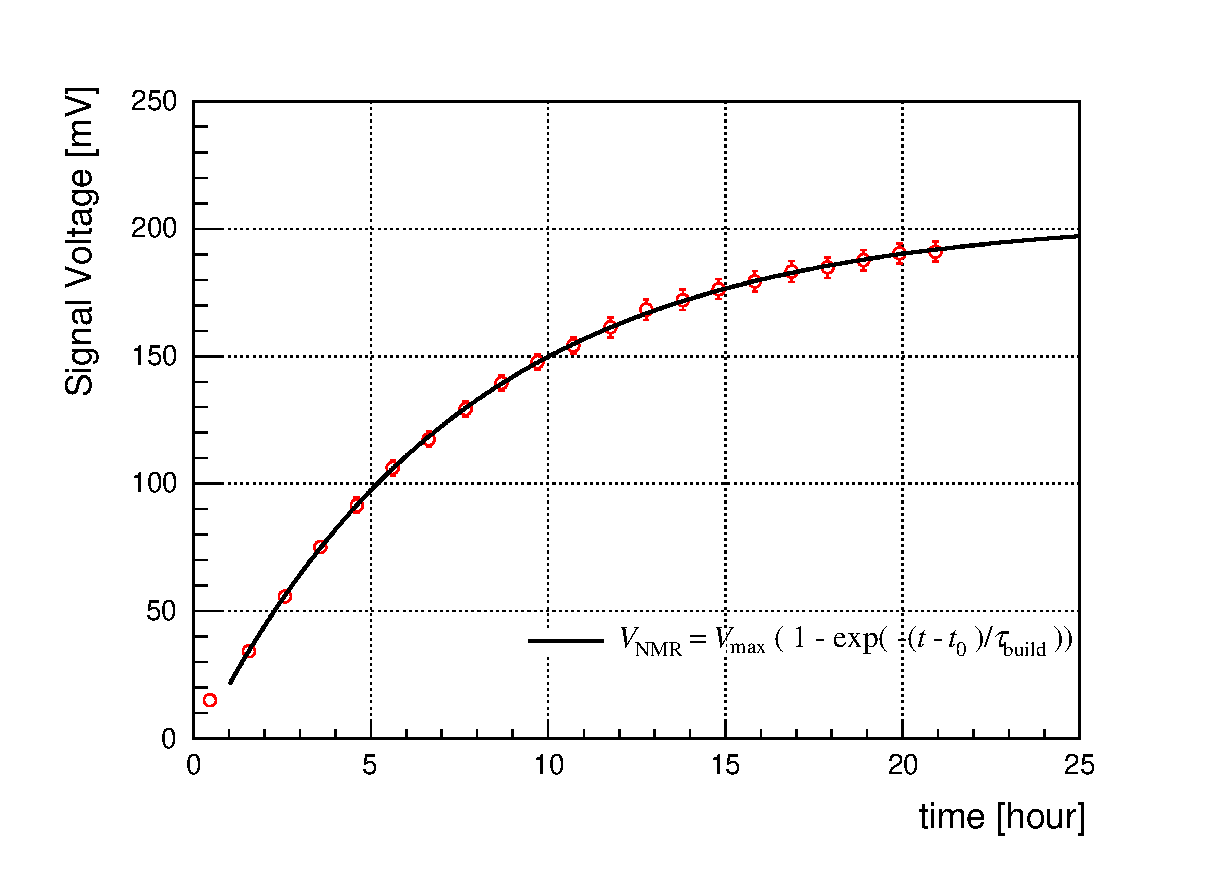
\includegraphics[clip, width=10cm]{./chap4/fig/NMR-buildup_1230.eps}\\
%  \caption{Kukiセルでの$^3$Heの偏極発展}
%  \label{NMR_build}
% \end{figure}


% %%%%%%%

% %% 4.1.2 %%
%   \subsection{偏極緩和}
% オーブンの温度を高温に保ちつつ、光ポンピングによって$^3$He原子核が偏極している状態でレーザーの照射を止めると、$^3$He原子核は偏極生成されなくなるために次第に偏極度が減少していく(偏極緩和)。光ポンピングがされなくなると、Rb原子の偏極は$^3$He原子核の偏極より十分速く緩和する。よって、$^3$He原子核の偏極度の時間変化(式(\ref{dP_3He/dt}))において$\overline{P}_{\rm Rb}=0$と見なせる。故に、この時の$^3$He原子核の偏極度は、次の式で書ける。
% %
% \begin{equation}
%  P_{\rm ^3He} = P_0 e^{-\Gamma_{\rm ^3He}'t}
%  \label{relax_hot}
% \end{equation}
% %
% ここで、$P_0$は$t=0$の時の$^3$He偏極度である。この条件における偏極緩和(高温偏極緩和)の立ち下りの時定数$\tau_{\rm hot}$は、式(\ref{relax_hot})より
% %
% \begin{equation}
%  \tau_{\rm hot} = \frac{1}{\Gamma_{\rm ^3He}'} = \frac{1}{X \cdot \gamma_{\rm SE}+\Gamma_{\rm ^3He}}
%  \label{tau_hot}
% \end{equation}
% %
% となる。よって$^3$Heの偏極緩和を測定し、$\tau_{\rm hot}$の値が求まれば、Rb蒸気との相互作用も含んだ$^3$He原子核の偏極緩和率$\Gamma_{\rm ^3He}'$を求めることができる。\\
%  Kukiセルを用いた場合の典型的な$^3$Heの高温偏極緩和の測定結果を図\ref{NMR_hotrelax}に示す。図\ref{NMR_hotrelax}における実線は、式(\ref{relax_hot})でフィッティングした結果である。またこの時、$t=0~{\rm h}$におけるNMR信号の大きさを$1$とした。フィッティングの結果、高温偏極緩和における時定数$\tau_{\rm hot}$は
% %
% \begin{equation}
%  \tau_{\rm hot} = 7.93 \pm 0.14~[{\rm h}]
% \end{equation}
% %
% となった。

% \begin{figure}[tbp]
%  \centering
%  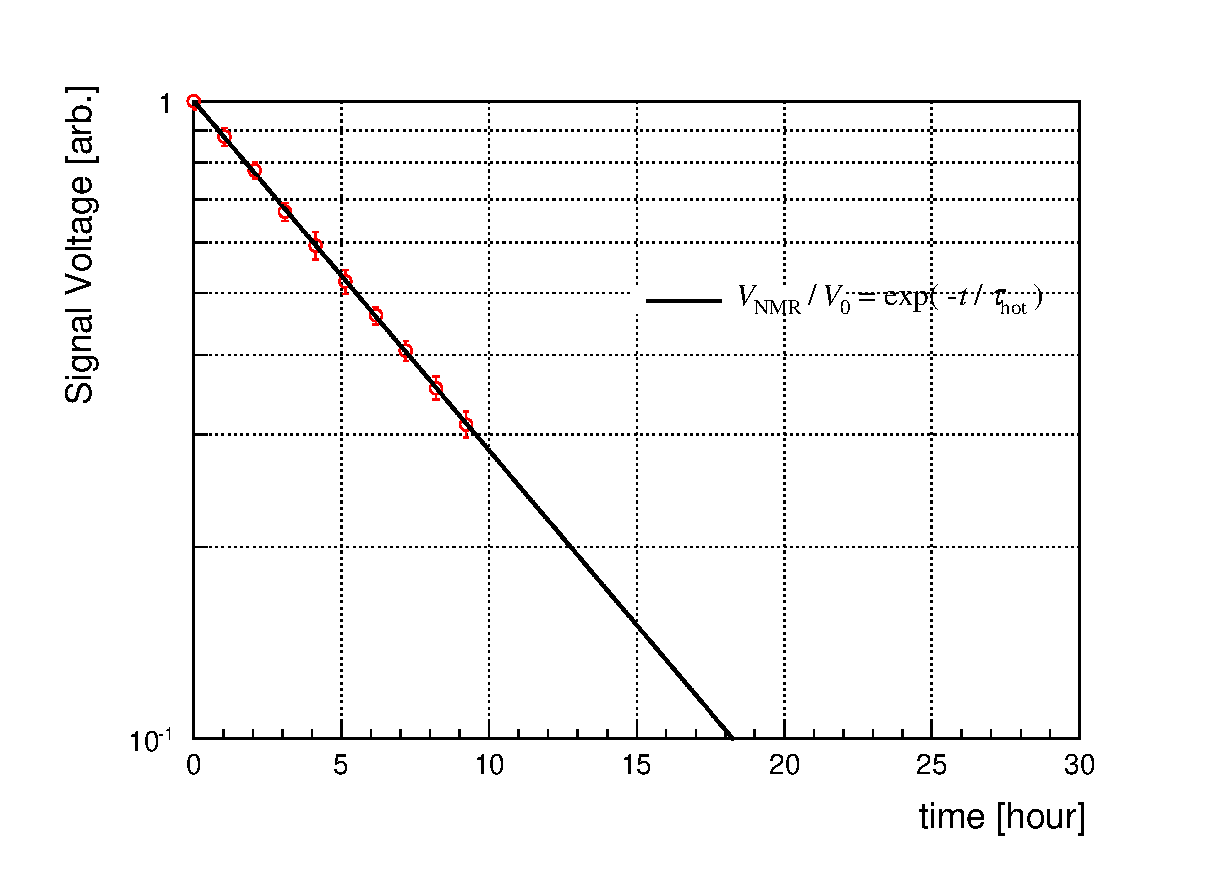
\includegraphics[clip, width=10cm]{./chap4/fig/NMR-hotrelax_1229.eps}\\
%  \caption{Kukiセルでの$^3$Heの高温偏極緩和}
%  \label{NMR_hotrelax}
% \end{figure}

% また光ポンピングによって$^3$He原子核が偏極している状態でレーザーの照射を止めると同時に、オーブンの加熱も止め、標的セル内の温度をRbの融点($39.31$℃)以下にすると、Rbが凝縮および凝固する。よって、Rb蒸気と$^3$He原子核との相互作用が無視できるようになる。この条件における偏極緩和(低温偏極緩和)の立ち下りの時定数$\tau_{\rm cold}$は
% %
% \begin{equation}
%  \tau_{\rm cold} = \frac{1}{\Gamma_{\rm ^3He}}
%  \label{tau_cold}
% \end{equation}
% %
% となり、Rb原子の数密度に依存しない$^3$He原子核の偏極緩和率を求めることができる。この低温偏極緩和における時定数$\tau_{\rm cold}$は、標的セル自体の性能を比較できるひとつの指標となる。\\
%  Kukiセルを用いた場合の典型的な$^3$Heの低温偏極緩和の測定結果を図\ref{NMR_coldrelax}に示す。図\ref{NMR_coldrelax}における実線は、式(\ref{relax_hot})と同様の形の式でフィッティングした結果である。またこの時、高温偏極緩和測定の場合と同様に$t=0~{\rm h}$におけるNMR信号の大きさを$1$とした。フィッティングの結果、低温偏極緩和における時定数$\tau_{\rm cold}$は
% %
% \begin{equation}
%  \tau_{\rm cold} = 9.73 \pm 0.11~[{\rm h}]
% \end{equation}
% %
% となり、高温偏極緩和の場合よりも$1.8~{\rm h}$程度長い緩和の時定数が得られた。よって、Rb蒸気と$^3$He原子核との相互作用による影響が無視されたことが確認できた。

% \begin{figure}[tbp]
%  \centering
%  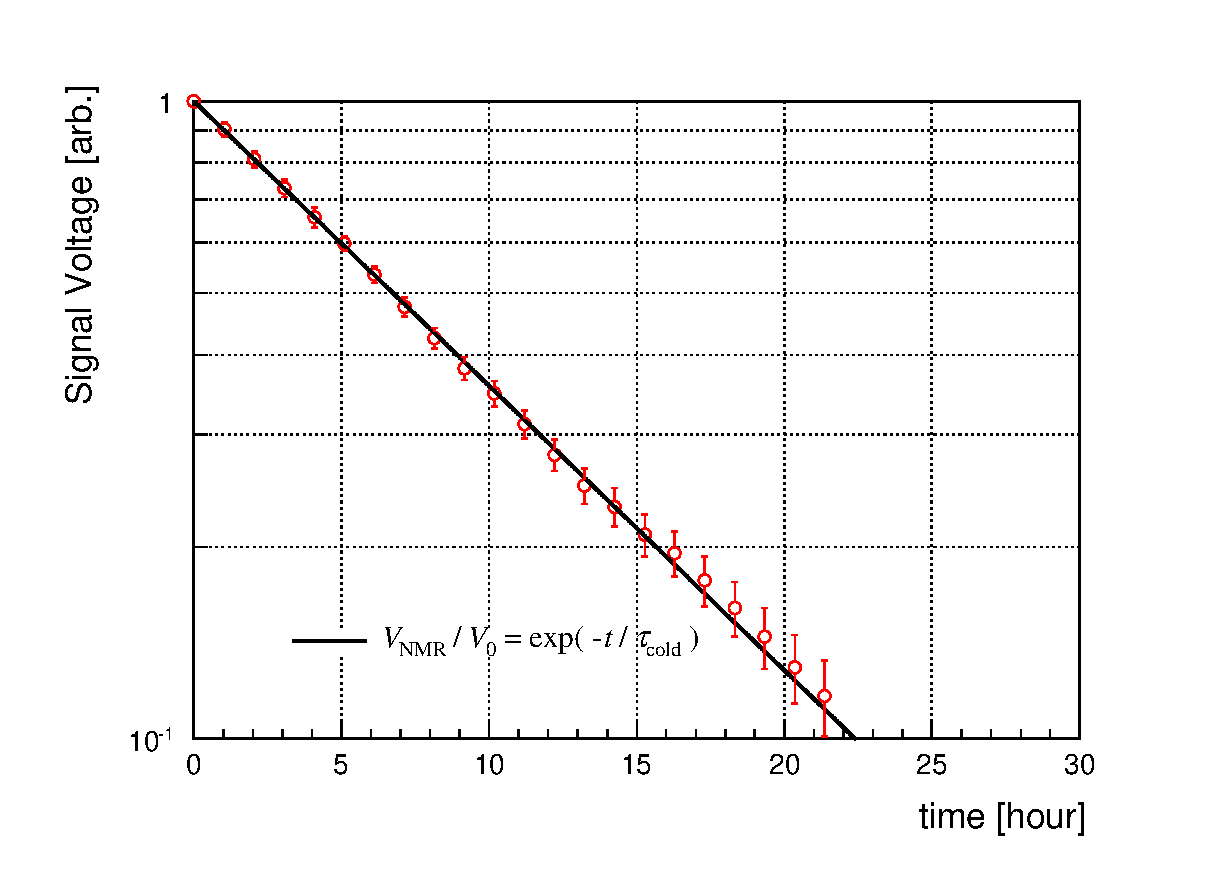
\includegraphics[clip, width=10cm]{./chap4/fig/NMR-coldrelax_1225.eps}\\
%  \caption{Kukiセルでの$^3$Heの低温偏極緩和}
%  \label{NMR_coldrelax}
% \end{figure}

 
% %%%%%%%

% %%%%%%%%%%

% %%%% 4.2 %%%%
%  \section{${}^3$He偏極度の絶対値較正}
% AFP-NMR法のみでは、$^3$He偏極度に比例した大きさのNMR信号しか得ることができない。$^3$He偏極度の絶対値を求めるために、第3章で述べたRbのESR周波数シフト測定による$^3$He偏極度測定システムを開発し、Rb-ESR測定装置を用いて$^3$He偏極度の測定を行った。以下の節では、$^3$He偏極度の測定結果およびNMR信号の較正について述べる。

% %% 4.2.1 %% 
%   \subsection{RbのESR周波数シフトによる${}^3$He偏極度測定}
% RbのESR周波数シフトは、$^3$He原子核の核スピンの向きが静磁場方向に対して平行または反平行それぞれにおけるRbのESR周波数を測定し、その差を取ることで得られる。$^3$He原子核の核スピンはAFP法によって反転させる。反転時にNMR測定も同時に行い、その時に得られたNMR信号を、RbのESR周波数シフトから求められる$^3$He偏極度に対応するものとする。\\
%  RbのESR周波数シフトの測定結果を図\ref{ESRfreq_mea}に示す。ESR周波数は、測定間隔$100~{\rm ms}$で$100$回測定(測定時間:$10$秒)を行うことで取得した。図\ref{ESRfreq_mea}において、$^3$He核スピンが上向き(静磁場に対して反平行)の場合は赤い三角、一方$^3$He核スピンが下向き(静磁場に対して平行)の場合は青い三角で示している。また、それぞれの点は10個毎に平均を取った値である。更に、図\ref{ESRfreq_mea}では偏極反転時に得られたNMR信号強度も示している。時間経過と共にNMR信号強度が減少し、それに従ってESR周波数シフトも小さくなっていることが分かる。これは円偏光のレーザーによる光ポンピングを測定中も行っているために、$^3$He原子核の核スピンの向きが静磁場と平行の時にレーザーによって$^3$Heの偏極を緩和(逆ポンピング)させていることによる。なるべく逆ポンピングによる$^3$He偏極度の緩和を抑制するために、一回のESR周波数の測定時間は$10$秒程度とした。測定結果から、およそ$2〜3~{\rm kHz}$程度のESR周波数シフトが得られた。

% \begin{figure}[tbp]
%  \centering
%  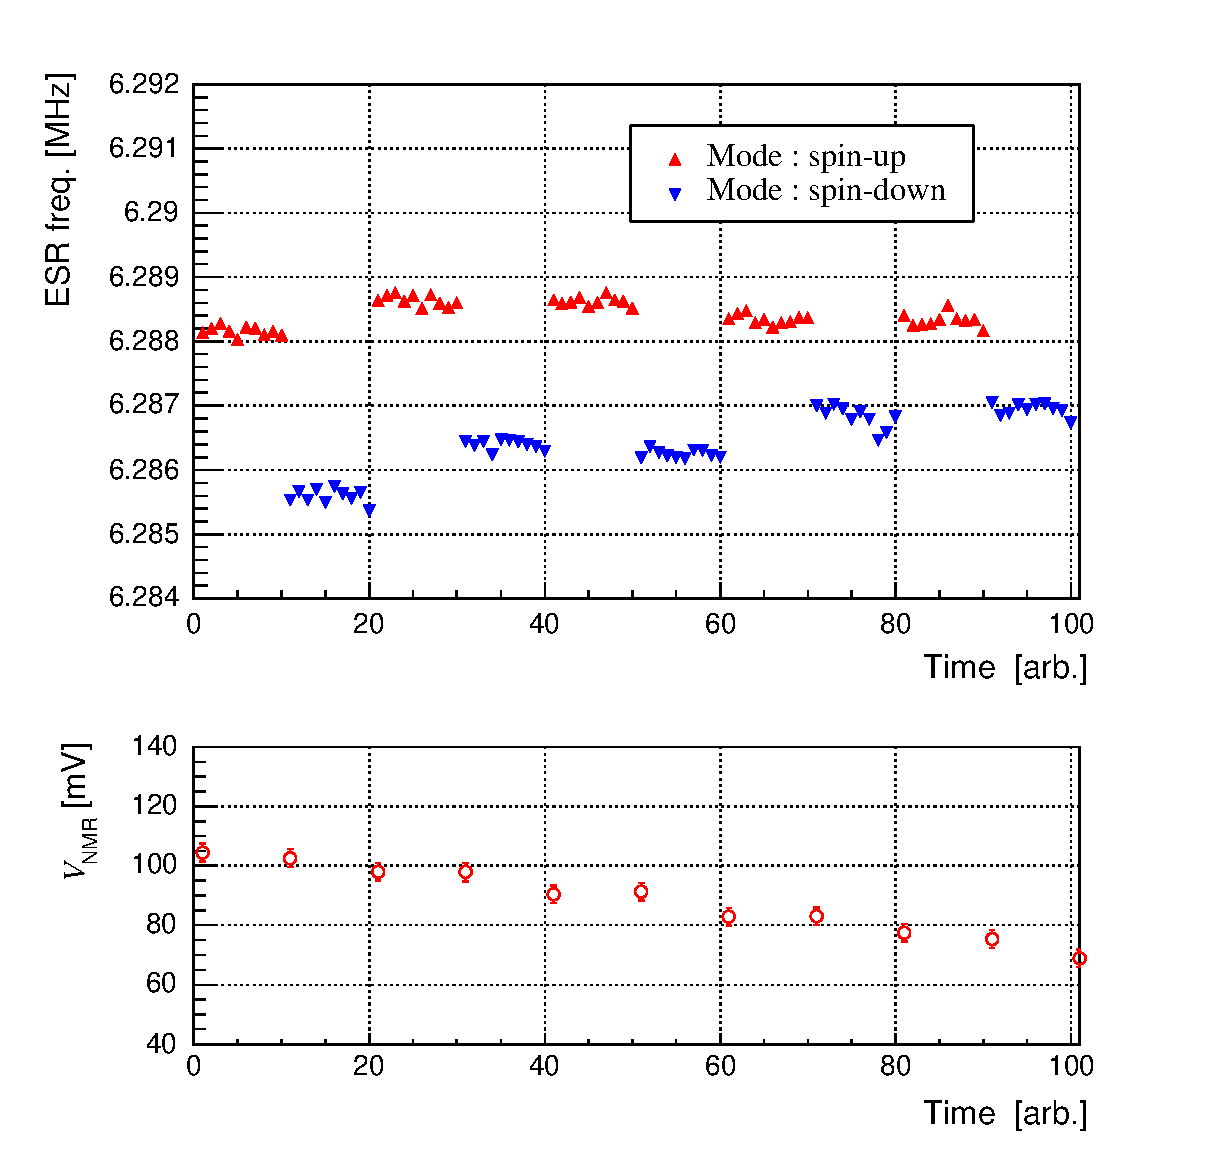
\includegraphics[clip, width=11cm]{./chap4/fig/ESRfreq_ave_Vnmr.eps}\\
%  \caption{典型的なESR周波数の測定データおよび偏極反転時のNMR信号強度}
%  \label{ESRfreq_mea}
% \end{figure}

% $\Delta \nu_{\rm ESR} = 3~{\rm kHz}$とした時の$^3$He偏極度を求める。RbのESR周波数シフト$\Delta \nu_{\rm ESR}$は、式(\ref{ESR_shift_updown})でも示したように
% %
%  \begin{eqnarray}
%   \Delta \nu_{\rm ESR}(m_F=\pm F) &=& \frac{2\mu_0}{3} \frac{\mu_{\rm B} g_e}{h(2I+1)} \left( 1\mp \frac{8I}{(2I+1)^2} \frac{\mu_{\rm B} g_e B_0}{hA_{\rm hfs}} \right)\kappa_0 \mu_{\rm K} [{\rm {}^3He}] (P_↑-P_↓) \nonumber \\
%   &\equiv& C_0 \kappa_0 [{\rm {}^3He}] (P_↑-P_↓) 
%   \label{Del_nu-P_3He} \\
%   C_0 &=&  \frac{2\mu_0}{3} \frac{\mu_{\rm K} \mu_{\rm B} g_e}{h(2I+1)} \left( 1\mp \frac{8I}{(2I+1)^2} \frac{\mu_{\rm B} g_e B_0}{hA_{\rm hfs}} \right)
%  \end{eqnarray}
% %
% となり、$^3$He偏極度と$^3$Heの数密度$[{\rm ^3He}]$の積に比例する。よって、標的セル内の$^3$Heガスの圧力を求める必要がある。3.1.1節で述べたように、$^3$Heガスを標的セルに封入する時のガス圧力はバラトロンゲージによって測定した。封入時のバラトロンゲージの出力電圧値は$1.36~{\rm V}$であった。よって、式(\ref{bara_calib})より液体窒素温度における標的セル内の$^3$Heガス圧力$Prs_{\rm ^3He}$は
% %
% \begin{equation}
%  Prs_{\rm ^3He} = \frac{1.36}{1.513 \times 10^{-3}} \simeq 898.9~[{\rm hPa}]
% \end{equation}
% %
% となる。よって、標的セル封入時のセル内の温度を$\sim 80~{\rm K}$程度とすると、バラトロンゲージによる測定結果から$^3$Heの数密度$[{\rm ^3He}]$は
% %
% \begin{equation}
%  [{\rm ^3He}] \simeq 8.17 \times 10^{19}~[{\rm cm^{-3}}]
%  \label{num_den_3He}
% \end{equation}
% %
% となった。よって、偏極反転による$^3$He原子核の減偏極が無いとすると、$\Delta \nu_{\rm ESR} = 3~{\rm kHz}$の時の$^3$He偏極度$P_{\rm ^3He}$は式(\ref{Del_nu-P_3He})より
% %
% \begin{eqnarray}
%  P_{\rm ^3He} &=& \frac{1}{2}(P_↑-P_↓) \nonumber \\
%  &=& \frac{\Delta \nu_{\rm ESR}}{2C_0 \kappa_0 [{\rm {}^3He}]} \simeq 7.39~[%]
% \end{eqnarray}
% %
% と求められる。

% %%%%%%%

% %% 4.2.2 %%
%   \subsection{NMR信号の較正}
% RbのESR周波数シフト測定の前後におけるNMR測定によって得られた信号強度から、NMR信号の$^3$He偏極度に対する較正を行った。NMR信号の較正は、測定したRbのESR周波数シフトから$^3$He偏極度を求め、その値とESR測定前後で測定し得られたNMR信号を平均した値とを対応させることで行った。これらの測定で得られたNMR信号強度$V_{\rm NMR}$とRbのESR周波数シフト$\Delta \nu_{\rm ESR}$および$^3$He偏極度$P_{\rm ^3He}$との関係を図\ref{ESRshift-Vnmr}に示す。この時、ESR周波数シフトの誤差$\delta \Delta \nu_{\rm ESR}$は、$^3$He核スピンが上向きの時のESR周波数の統計誤差$\delta \nu_{\rm up}$および$^3$He核スピンが下向きの時のESR周波数の統計誤差$\delta \nu_{\rm down}$を用いて
% %
% \begin{equation}
%  \delta \Delta \nu_{\rm ESR} = \sqrt{(\delta \nu_{\rm up})^2 + (\delta \nu_{\rm down})^2}
% \end{equation}
% %
% と表される。またNMR信号強度の誤差は読み取り誤差としては$3~{\rm mV}$程度であった。

% \begin{figure}[tbp]
%  \centering
%  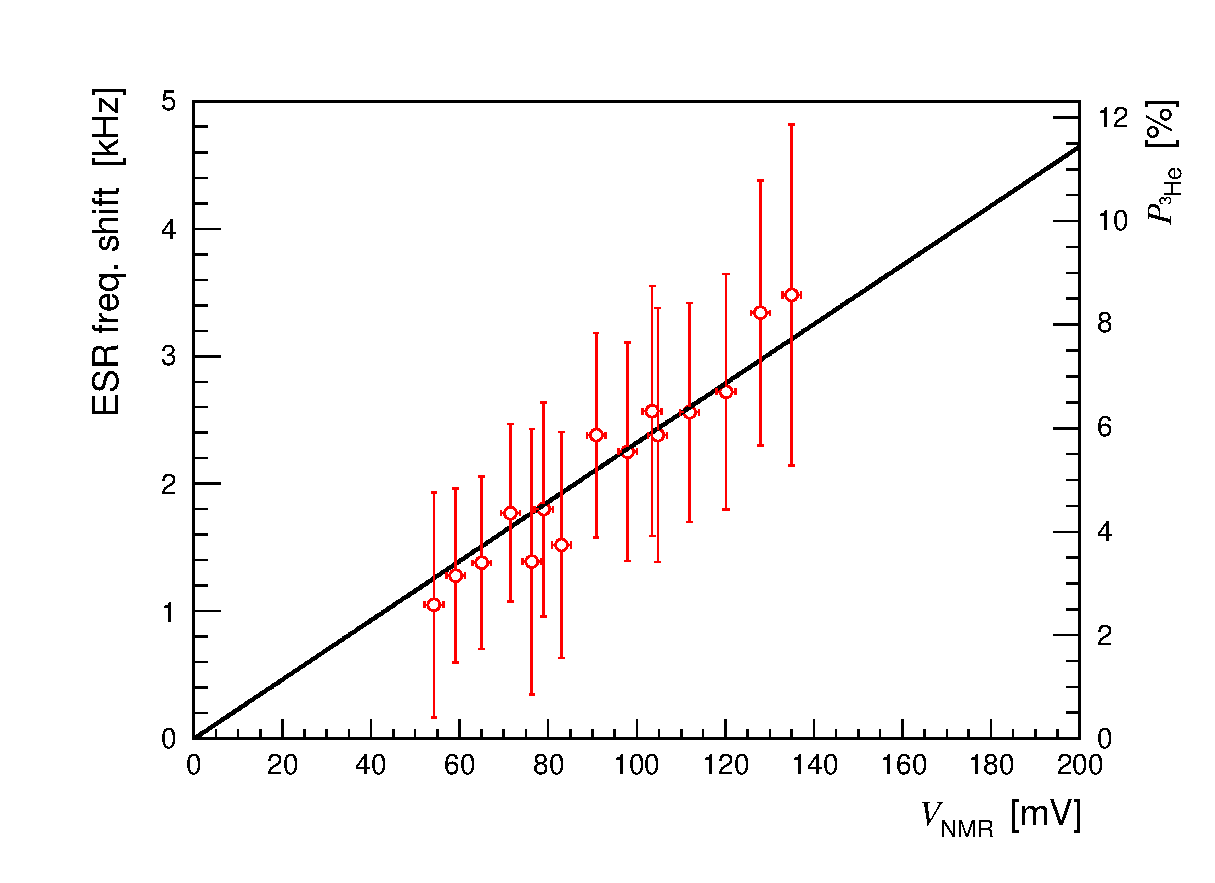
\includegraphics[clip, width=10cm]{./chap4/fig/ESRfreq-NMRsignal_P_3He.eps}\\
%  \caption{ESR周波数シフト、NMR信号強度および$^3$He偏極度との関係図}
%  \label{ESRshift-Vnmr}
% \end{figure}

% 図\ref{ESRshift-Vnmr}において、実線は原点を通る一次関数でフィッティングをした結果である。フィッティング結果から、NMR信号強度$V_{\rm NMR}$および$^3$He偏極度$P_{\rm ^3He}$は
% %
% \begin{equation}
%  P_{\rm ^3He}~[%] = (5.72 \pm 0.61) \times 10^{-2} V_{\rm NMR}~[{\rm mV}]
%  \label{rel_P_3He-Vnmr}
% \end{equation}
% %
% と対応付けられた。

% %%%%%%%

% %%%%%%%%%%
 
 